\section*{Resultados}
Los resultados que obtuvimos son los siguientes:
\begin{enumerate}[I.]
    \item De las gráficas obtenidas al ordenar las entidades federativas, observamos que Sinaloa tiene un crecimiento demasiado desproporcionado a las demás.
    \item Observando las correlaciones que obtuvimos podemos observar que el volumen y valor están muy relacionados entre sí, así como el número de sacrificados y su precio. \newpage 
    \item Y por último la predicción que hicimos del año, si bien no es la misma, podemos observar que están en el mismo rango de valores y son casi idénticos en este último.
\begin{figure}[!h]
    \centering
    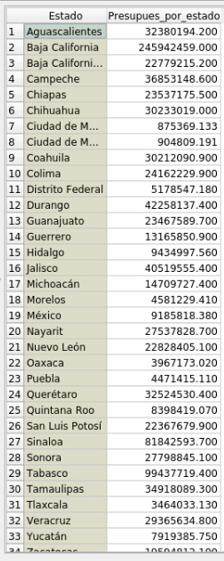
\includegraphics[width = 6 cm]{prep.jpeg}
    \caption{Presupuesto por estado}
    \label{diagrama}
\end{figure}
\newline
De la tabla que fue mostrada podemos ver cuál es la propuesta de presupuesto para cada uno de los estados. Y otra manera de visualizarlo es con un gráfico de barras: 
\begin{figure}[h]
    \centering
    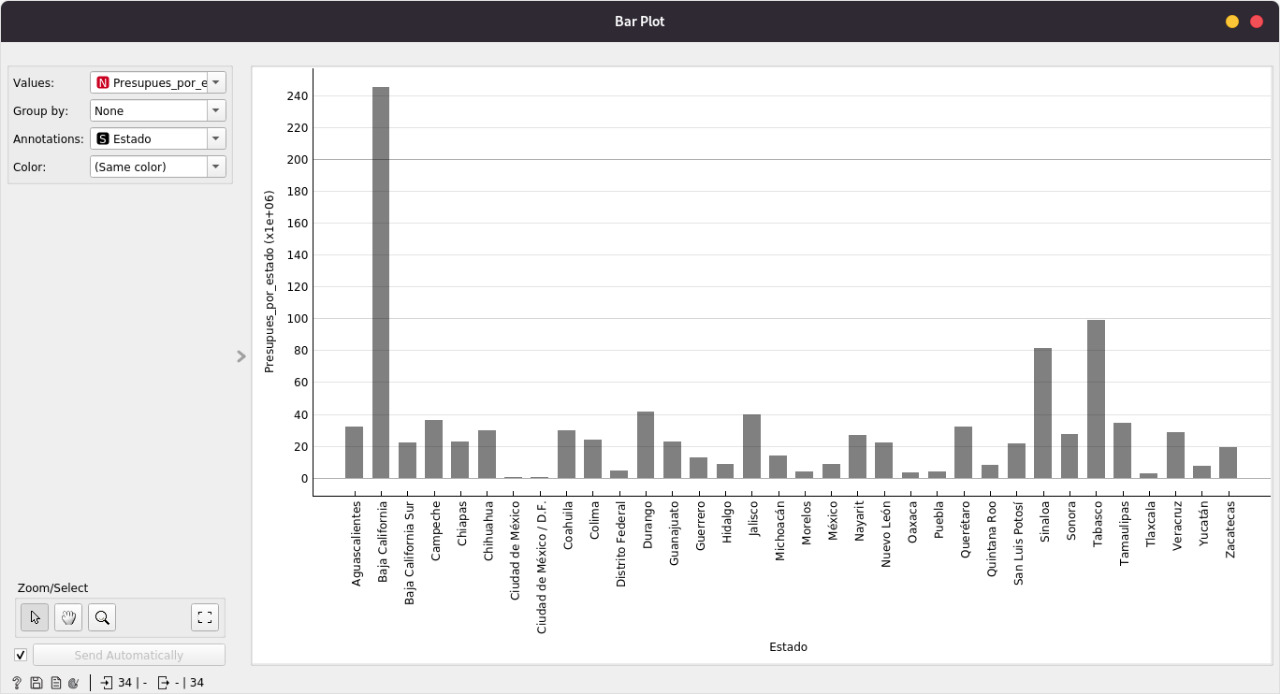
\includegraphics[width = 12 cm]{imagenes/grafica.jpeg}
    \caption{Grafico de barras de presupuesto por estado.}
    \label{diagrama}
\end{figure}


\end{enumerate}